\chapter{Resultados e Discussão}

\section{Estruturas de Linhas de Defeitos}

Os resultados referentes as simulações das estruturas com padrões de linhas demonstram que os defeitos de Stone-Wales afetam de maneira positiva a eficiência da estrutura na catálise de hidrogênio.\
As figuras \ref{line1} e \ref{line2}, exibem uma melhora do comportamento catalítico nos sítios localizados na região central dos defeitos, e, em especial, em regiões de união entre os defeitos.

\begin{figure}[H]
    \centering
    
\includegraphics[width=0.9\textwidth]{/home/geedai/Desktop/tcc/figuras/lines.jpg}
    \caption{Estruturas com defeitos de padrões de linhas, organizada por espessura da linha no eixo vertical, e distância entre linhas no eixo horizontal. A variação da energia livre de Gibbs é representada pelo mapa de cores.}
    \label{line1}
\end{figure}

\begin{figure}[H]
    \centering
    
\includegraphics[width=0.9\textwidth]{/home/geedai/Desktop/tcc/figuras/linesbottom.jpg}
    \caption{Estruturas com defeitos de padrões de linhas, organizada por espessura da linha no eixo vertical, e distância entre linhas no eixo horizontal. A variação da energia livre de Gibbs é representada pelo mapa de cores.}
    \label{line2}
\end{figure}

Além da mudança clara do $\Delta G$ em relação a estrutura pristina do grafeno, é notável a diferença entre os dois lados da folha de grafeno modificada. A adição de um único defeito mantém a simetria entre os dois lados da folha, mas\
a união entre dois defeitos cria um efeito de rugosidade, como apresentado na figura \ref{buckling} que cria uma diferença no $\Delta G$ em cada lado da mesma estrutura.

\begin{figure}[H]
    \centering
    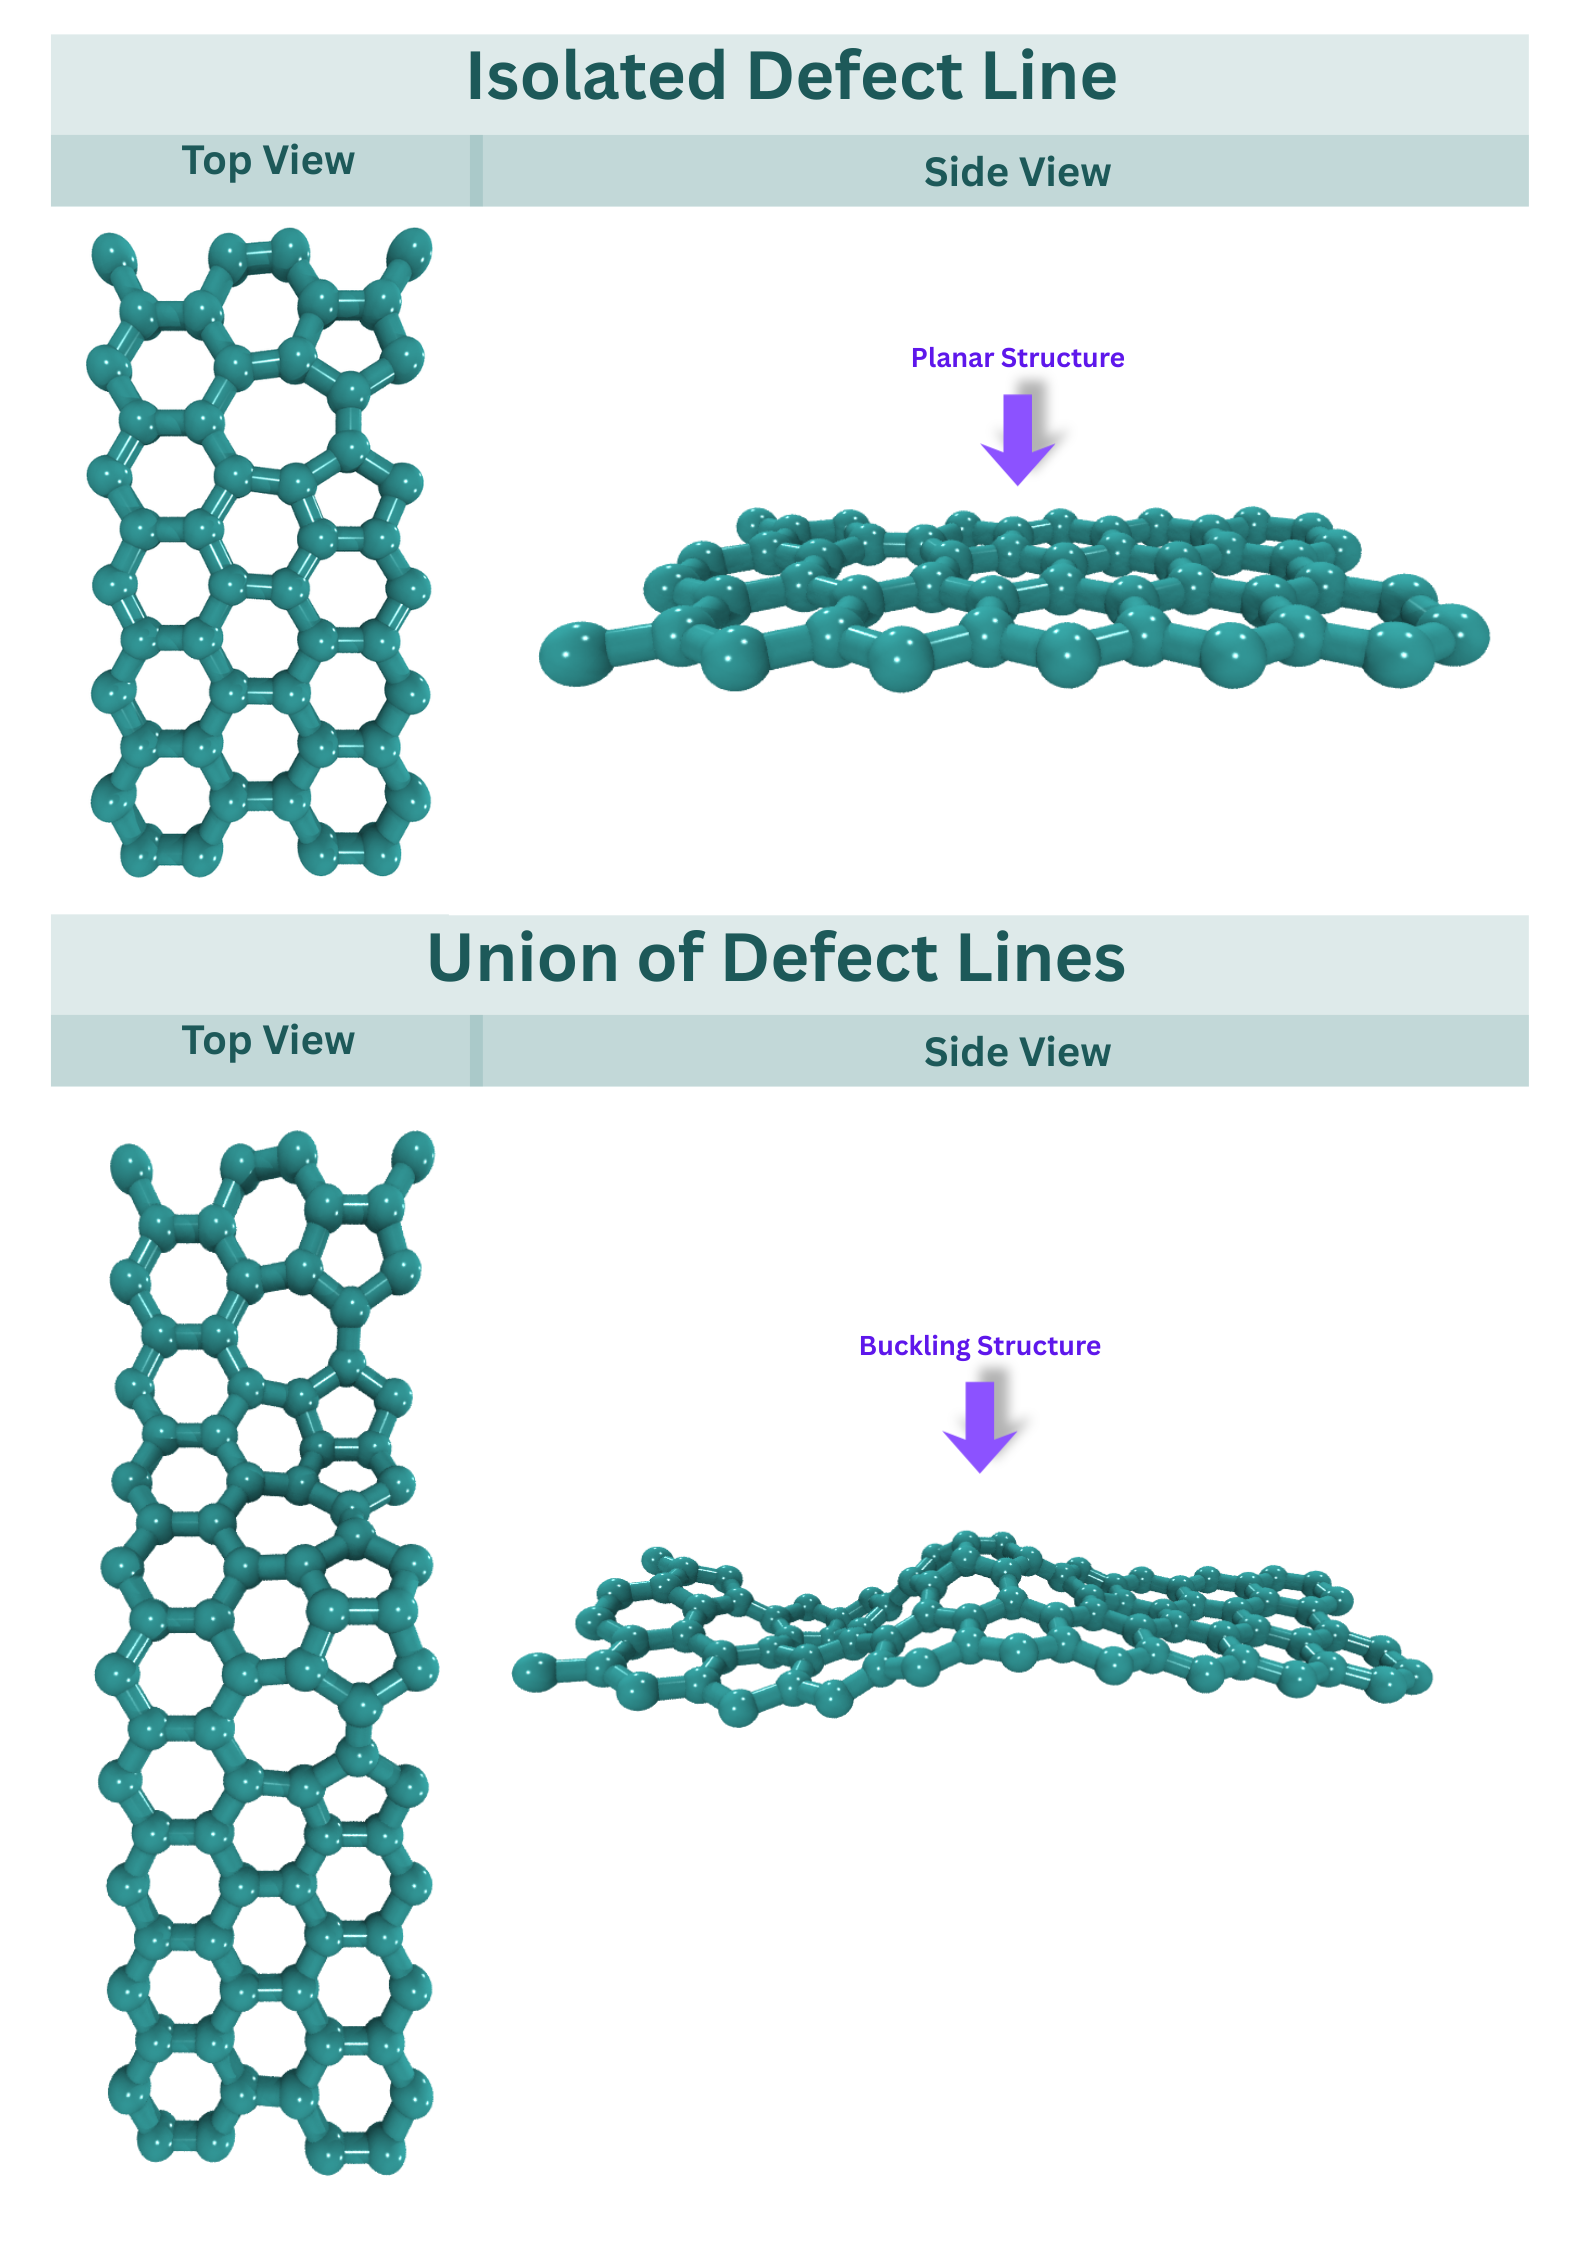
\includegraphics[width=0.9\textwidth]{figuras/Buckling.png}
    \caption{Acima estrutura com uma linha de defeito isolada, e abaixo uma estrutura com união de linhas de defeito.}
    \label{buckling}
\end{figure}

\section{Estruturas de Shuriken}

As estruturas do tipo shuriken-3 e 4 apresentaram redução no valor da energia livre de Gibbs em relação ao grafeno pristino em certos átomos localizados nos aneis dos defeitos de Stone-Wales, formando alguns sítios próprios para a catálise.\
Já o shuriken-6 apresentou uma intensa mudança do $\Delta G$, chegando a valores negativos, e muitos sítios com $\Delta G$ proximos de zero.

Todas as estruturas do tipo shuriken apresentaram efeitos de curvatura em sua superfície que criam as diferenças do $\Delta G$ em cada lado, como apresentado na figura \ref{sks}.
\begin{figure}[H]
    \centering
    
\includegraphics[width=0.9\textwidth]{/home/geedai/Desktop/tcc/figuras/shurikens_dg.png}
    \caption{Estruturas do tipo shuriken com mapa de cor do $\Delta G$ em cada lado da superfície.}
    \label{sks}
\end{figure}

\section{Analise da Curvatura}

Foi observado que a adição de defeitos de Stone-Wales isolados na estrutura do grafeno mantém a superfície plana e portanto simétrica em relação ao eixo z. Por outro lado, a uniao de defeitos gera rugosidade na superfície, criando uma diferença de energia livre de adsorção de hidrogênio em cada lado.\
Dessa forma, faz sentido verificar como a diferença de $\Delta G$ em cada lado é afetada pela curvatura local da superfície.

A relação entre a diferença de $\Delta G$ e a curvatura é exibida na figura \ref{curva1} e \ref{curva2}, apresentando uma grande correlação linear entre esses dois fatores. 

\begin{figure}[H]
    \centering
    
\includegraphics[width=0.9\textwidth]{/home/geedai/Desktop/tcc/figuras/curvature_lines.png}
    \caption{Diferença de $\Delta G$ em cada lado da superfície para cada sítio pela curvatura local no sítio para estruturas de linha.}
    \label{curva1}
\end{figure}

\begin{figure}[H]
    \centering
    
\includegraphics[width=0.9\textwidth]{/home/geedai/Desktop/tcc/figuras/curvature_shuriken.png}
    \caption{Diferença de $\Delta G$ em cada lado da superfície para cada sítio pela curvatura local no sítio para estruturas de shuriken.}
    \label{curva2}
\end{figure}

Os coeficientes angulares das retas ajustadas são A = 4.065 ± 0.144 para estruturas de linhas e A = 3.655 ± 0.319 para estruturas shuriken.


\section{Comparação Entre DFTB e DFT}

A comparação entre os o método do DFT e o DFTB é apresentada na figura \ref{dftb_dft}, em que cada ponto é o valor do $\Delta G$ de um sítio em um dos lados da superfície das estruturas de linha e shuriken. A linha reta se refere aos valores em que os dois métodos concordam, enquanto que valores longe da linha apresentam discrepância entre os métodos.

É evidente que alguns pontos apresentam um grande distânciamento da reta identidade. Contudo, a grande maioria dos pontos seguem a mesma tendência da reta, mas com uma certa defasagem em relação ao eixo vertical.\
Isso sugere que os métodos concordam entre sí quanto ao comportamento do sistema, mas discordam dos valores com um erro quadrático médio (RMSE) de 0.4 eV.

\begin{figure}[H]
    \centering
    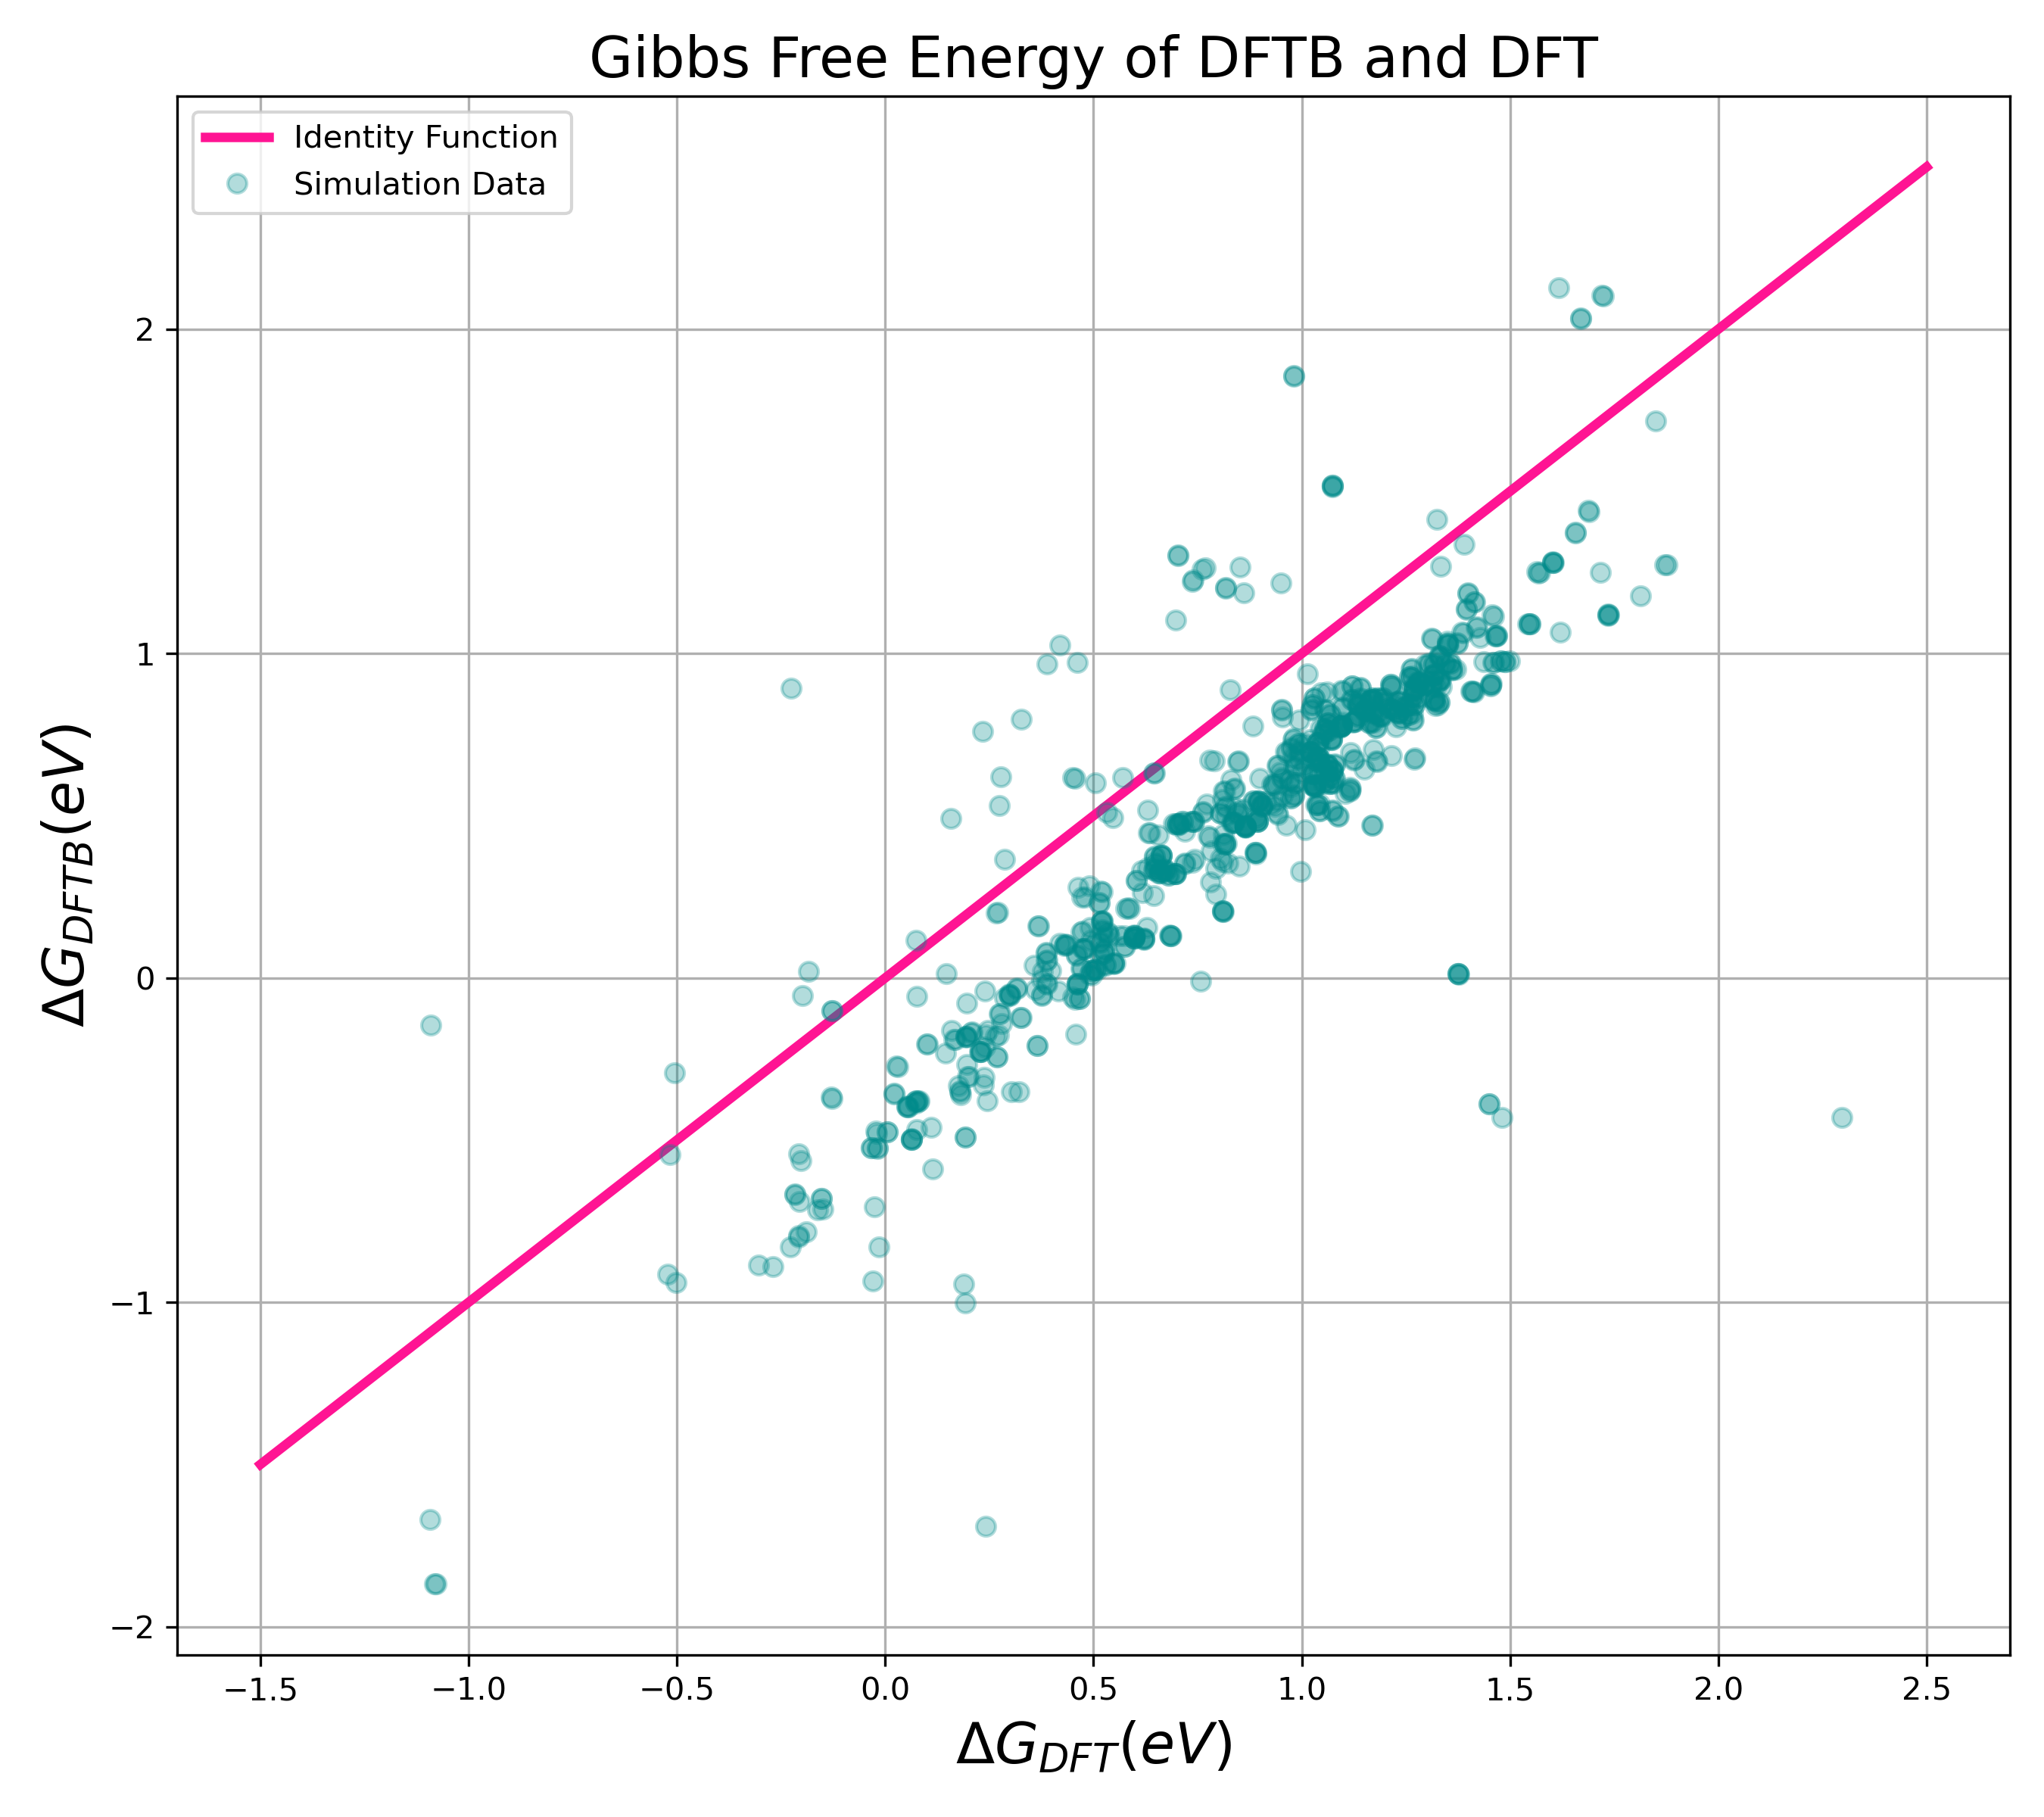
\includegraphics[width=0.9\textwidth]{figuras/dftb_dft.png}
    \caption{Valores de $\Delta G$ para os sítios das estruturas de linha e shuriken utilizando os métodos de DFTB (eixo y) e DFT (eixo x). A linha rosa é a reta identidade.}
    \label{dftb_dft}
\end{figure}

Como a relação entre o DFT e o DFTB é aparentemente linear, pode-se realizar uma correção desse tipo ajustando uma reta no gráfico. Isso é apresentado na figura \ref{dftb_fit},\
onde a reta é $\Delta G_{DFT} = 0.767 \Delta G_{DFTB} + 0.469$ eV. Contudo, o RMSE para o ajuste é de $0.243$, fazendo com que os valores calculados utilizando o DFTB possuem um desvio muito grande em relação ao tamanho da faixa ideal de $\Delta G$.

\begin{figure}[H]
    \centering
    
\includegraphics[width=0.9\textwidth]{dftb_dft_fit.png}
    \caption{Valores de $\Delta G$ para os sítios das estruturas de linha e shuriken utilizando os métodos de DFTB (eixo x) e DFT (eixo y). A linha laranja é um ajuste linear, e o sombreamento laranja é a região de incerteza.}
    \label{dftb_fit}
\end{figure}

